\section{GStreamer}

\begin{frame}{Introduction}
  \begin{itemize}
  \item \code{Gstreamer} is an open-source multimedia framework that
    provides a pipeline-based architecture for handling multimedia
    data such as audio and video.
  \item \url{https://gstreamer.freedesktop.org/}
  \item \code{GStreamer} provides a unified framework for handling
    various multimedia formats and tasks.
  \item It supports a wide range of codecs, formats, and protocols.
  \item Its modular architecture supports plugins and allows the
    addition of new elements, codecs, and functionality.
  \end{itemize}
\end{frame}

\begin{frame}{Architecture}
  \begin{itemize}
  \item \code{GStreamer} is object oriented, it adheres to the
    \code{GObject} model of \code{GLib 2.0}.
  \item The main object is an \code{Element}. Each element has a
    specific function e.g. reading, writing, encoding or decoding
    data. By chaining elements, its is possible to create a
    \code{pipeline} to achieve a task.
  \item Elements communicate with each other through \code{pads}. A
    pad is a connection point that can be an input (\code{sink}) or
    output (\code{source}). Elements are linked by connecting pads. A
    pad can restrict the type of data that flows through it. Links are
    only allowed between two pads when the allowed data types
    (capabilities) of the two pads are compatible.
  \item A \code{bin} is a container for a collection of elements. It
    can be controlled just like an element
  \item A \code{pipeline} is a top level bin. Allowing to control and
    synchronize all its children.
  \end{itemize}
\end{frame}

\begin{frame}{Example}
  \begin{center}
    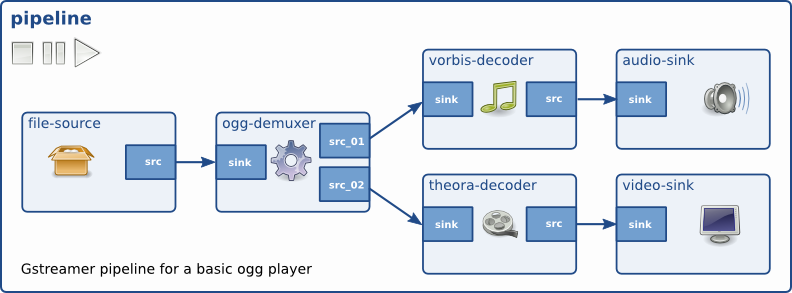
\includegraphics[width=\textwidth]{slides/audio-gstreamer/simple-player.png}\\
    {\textit Example of a GStreamer pipeline}
  \end{center}
\end{frame}

\begin{frame}{Plugins}
  \begin{itemize}
  \item Plugins are selfcontained libraries loaded at runtime.
  \item All relevant aspects of plugins can be queried at run-time.
  \item All the properties can be set using the GObject properties, there is no need for header files.
  \item Core plugins:
    \begin{itemize}
    \item audiotestsrc, videotestsrc: Generates test audio or video
      patterns.
    \item autoaudiosink, autovideosink: Automatically selects an
      output and plays audio or displays video.
    \item filesrc, filesink: Read from and write to files.
    \item decodebin: Automatically selects and configures decoders
      based on media content.
    \item playbin: Automatically plays audio and video from a location
    \end{itemize}
  \end{itemize}
\end{frame}

\begin{frame}{Useful Plugins}
  \begin{center}
  \fontsize{8}{9}\selectfont
  \begin{tabularx}{13cm}{l|l|X}
    alsasink & Sink Audio & Output to a sound card via ALSA \\
    alsasrc & Source Audio & Read from a sound card via ALSA \\
    audioconvert & Filter Converter Audio & Convert audio to different formats \\
    audiodynamic & Filter Effect Audio & Compressor and Expander \\
    audiolatency & Audio Util & Measures the audio latency between the source and the sink \\
    audioloudnorm & Filter Effect Audio & Normalizes perceived loudness of an audio stream \\
    audiomixmatrix & Filter Audio & Mixes a number of input channels
    into a number of output channels according to a transformation
    matrix \\
    audioresample & Filter Converter Audio & Resamples audio \\
    clocksync & Generic &Synchronise buffers to the clock \\
    dtmfdetect & Filter Analyzer Audio & This element detects DTMF tones \\
    dtmfsrc & Source Audio & Generates DTMF tones \\
    jackaudiosink & Sink Audio & Output audio to a JACK server \\
    jackaudiosrc & Source Audio & Captures audio from a JACK server \\
  \end{tabularx}
  \end{center}
\end{frame}

\begin{frame}{Command line tools}
  \begin{itemize}
  \item \code{gst-inspect-1.0} is a tool that prints out information
    on GStreamer plugins and elements.
  \item Without any arguments, it prints a list of all plugins and
    elements it knows about.
  \item \code{gst-launch-1.0} builds and runs a GStreamer pipeline
    on GStreamer plugins and elements.
  \item It takes a pipeline description as an argument, this is a list
    of elements separated by exclamation marks (!). Properties may be
    appended to elements in the form property=value.
  \item \code{gst-launch-1.0} is a tool useful for debugging but
    shouldn't be used as a standalone application.
  \item For example, to play an ogg file using ALSA:
    \code{gst-launch-1.0 filesrc location=music.ogg ! oggdemux ! vorbisdec !
    audioconvert ! audioresample ! alsasink}
  \end{itemize}
\end{frame}

\begin{frame}{Debugging}
  \begin{itemize}
  \item \code{gst-launch-1.0} has a \code{-v} option to make it
    verbose
  \item GStreamer also uses the \code{GST_DEBUG} environment variable.
    It takes a debug level from 0 (none) to 9 (memdump). This can also
    be filtered by element and categories. For example,
    \code{GST_DEBUG=2,audiotestsrc:6}, will use level 6 for the
    \code{audiotestsrc} element, and 2 for all the others.
  \item When \code{GST_DEBUG_DUMP_DOT_DIR} environment variable is set
    and point to a folder, \code{gst-launch-1.0} will create a
    \code{.dot} file at each state change. \code{graphviz} can then be
    used to generate a graph.
    \begin{itemize}
    \item \code{gst-launch-1.0 filesrc location=Media/test_32_16.wav !
      decodebin ! alsasink}
    \item \code{dot -Kfdp -Tpng -o pipeline.png 0.00.00.021721659-gst-launch.PAUSED_PLAYING.dot}
    \end{itemize}
  \end{itemize}
\end{frame}

\begin{frame}{Debugging - graph}
  \begin{center}
    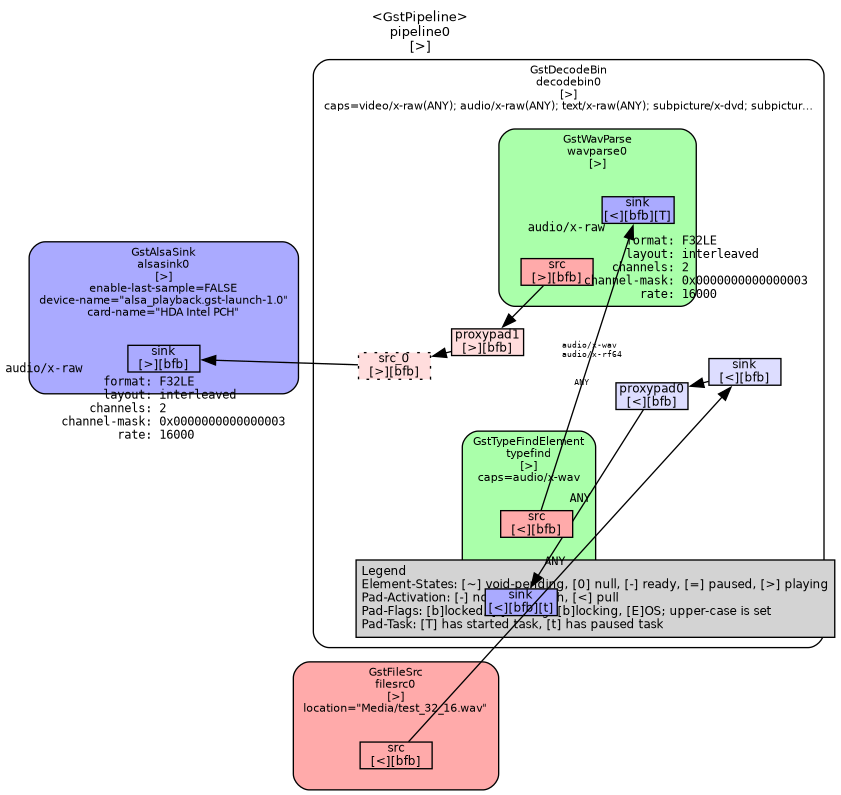
\includegraphics[height=0.8\textheight]{slides/audio-gstreamer/pipeline.png}\\
  \end{center}
\end{frame}

\begin{frame}{Resources}
  \begin{itemize}
  \item Documentation:
    \url{https://gstreamer.freedesktop.org/documentation/}. This
    includes documentation of the API to write application and
    plugins.
  \item Plugin list:
    \url{https://gstreamer.freedesktop.org/documentation/plugins_doc.html}
  \end{itemize}
\end{frame}

\setupdemoframe
{Gstreamer}
{
  \begin{itemize}
  \item Inspect plugins and elements using \code{gst-inspect}
  \item Prepare multiple pipelines with \code{gst-launch}
  \end{itemize}
}
